% BLOCK C: THE LABORATORY OF LIVING - Professional LaTeX Edition
\documentclass[12pt,openany]{book}

% Premium Typography Packages
\usepackage[utf8]{inputenc}
\usepackage[T1]{fontenc}
\usepackage{ebgaramond} % Elegant Garamond font
\usepackage[tracking=true, letterspace=50]{microtype} % Microtypography
\usepackage{lettrine} % Drop caps

% Page Layout - 6x9 book
\usepackage[paperwidth=6in, paperheight=9in,
            top=0.85in, bottom=0.85in,
            inner=0.85in, outer=0.7in]{geometry}

% Color Palette
\usepackage{xcolor}
\definecolor{creambg}{HTML}{E8E4DC}
\definecolor{richblack}{HTML}{1A1A1A}
\definecolor{deepslate}{HTML}{2F4F4F}
\definecolor{brightcyan}{HTML}{00CED1}
\definecolor{warmamber}{HTML}{FFB347}
\definecolor{softgray}{HTML}{8B8B8B}

% Graphics and Artwork
\usepackage{graphicx}
\usepackage{tikz}
\usetikzlibrary{positioning, decorations.pathmorphing}

% Chapter and Section Styling
\usepackage{titlesec}
\usepackage{fancyhdr}

% Links and Metadata
\usepackage[hidelinks]{hyperref}
\hypersetup{
    pdftitle={Block C: The Laboratory of Living},
    pdfauthor={Brandon Mills and Jesse Doherty},
    pdfsubject={Self-Actualization},
    pdfkeywords={consciousness, self-actualization, transformation}
}

% Paragraph formatting
\usepackage{parskip}
\setlength{\parindent}{1.5em}
\setlength{\parskip}{0pt}

% Page color
\pagecolor{creambg}

% Header/Footer
\pagestyle{fancy}
\fancyhf{}
\fancyhead[LE,RO]{\small\color{softgray}\textit{Block C • The Laboratory of Living}}
\fancyfoot[C]{\color{richblack}\thepage}
\renewcommand{\headrulewidth}{0.3pt}
\renewcommand{\footrulewidth}{0.3pt}
\renewcommand{\headrule}{\hbox to\headwidth{\color{softgray!30}\leaders\hrule height \headrulewidth\hfill}}
\renewcommand{\footrule}{\hbox to\headwidth{\color{softgray!30}\leaders\hrule height \footrulewidth\hfill}}

% Chapter formatting with geometric design
\titleformat{\chapter}[display]
  {\normalfont\huge\bfseries\color{richblack}\centering}
  {}
  {0pt}
  {%
    \vspace*{0.8in}%
    % Geometric decoration
    
\begin{tikzpicture}[remember picture, overlay]
      \draw[line width=1.2pt, color=deepslate] (-2.5,0.5) -- (-2.5,-0.5);
      \draw[line width=1.2pt, color=deepslate] (-2.5,0.5) -- (-2.2,0.5);
      \draw[line width=1.2pt, color=deepslate] (-2.5,-0.5) -- (-2.2,-0.5);
      \draw[line width=1.2pt, color=deepslate] (2.5,0.5) -- (2.5,-0.5);
      \draw[line width=1.2pt, color=deepslate] (2.5,0.5) -- (2.2,0.5);
      \draw[line width=1.2pt, color=deepslate] (2.5,-0.5) -- (2.2,-0.5);
      \fill[brightcyan] (0,0) -- (0.15,0.15) -- (0,0.3) -- (-0.15,0.15) -- cycle;
      \foreach \angle in {0,45,...,315} {
        \fill[warmamber] ({0.4*cos(\angle)},{0.4*sin(\angle)}) circle (1.5pt);
      }
    \end{tikzpicture}%
    \vspace{0.4in}%
    \MakeUppercase
  }
  [\vspace{0.3in}{\color{deepslate}\titlerule[2pt]}]

% Section formatting
\titleformat{\section}
  {\normalfont\Large\bfseries\color{deepslate}}
  {}
  {0pt}
  {
\begin{tikzpicture}
    \draw[line width=2.5pt, color=deepslate] (0,0) -- (0,1.2);
    \draw[line width=1pt, color=brightcyan] (0,0) -- (-0.2,0);
    \draw[line width=1pt, color=brightcyan] (0,1.2) -- (-0.2,1.2);
  \end{tikzpicture}\hspace{0.3in}}

% Subsection formatting
\titleformat{\subsection}
  {\normalfont\large\bfseries\color{richblack}}
  {}
  {0pt}
  {}
  [\vspace{-0.2in}{\color{brightcyan}\titlerule[1.2pt]}]

% Pull quote environment
\usepackage{mdframed}
\newmdenv[
  linewidth=0pt,
  leftline=true,
  linecolor=brightcyan,
  innerleftmargin=0.5in,
  innerrightmargin=0.5in,
  innertopmargin=0.3in,
  innerbottommargin=0.3in,
  backgroundcolor=brightcyan!8,
  leftmargin=0.5in,
  rightmargin=0.5in,
  skipabove=0.4in,
  skipbelow=0.4in,
  innerlinewidth=4pt
]{pullquote}

% No headers/footers on chapter pages
\fancypagestyle{plain}{%
  \fancyhf{}%
  \renewcommand{\headrulewidth}{0pt}%
  \renewcommand{\footrulewidth}{0pt}%
}

\begin{document}

% Remove page numbers from first page
\thispagestyle{empty}

% ============================================================================
% TITLE PAGE
% ============================================================================
\begin{titlepage}
\pagecolor{creambg}
\centering
\vspace*{0.6in}

% Geometric design

\begin{tikzpicture}
  \draw[line width=1.2pt, color=deepslate] (-3,-0.8) -- (-3,0.8);
  \draw[line width=1.2pt, color=deepslate] (-3,-0.8) -- (-2.6,-0.8);
  \draw[line width=1.2pt, color=deepslate] (-3,0.8) -- (-2.6,0.8);
  \draw[line width=1.2pt, color=deepslate] (3,-0.8) -- (3,0.8);
  \draw[line width=1.2pt, color=deepslate] (3,-0.8) -- (2.6,-0.8);
  \draw[line width=1.2pt, color=deepslate] (3,0.8) -- (2.6,0.8);
  \draw[line width=1.2pt, color=brightcyan] (0,0) circle (0.2);
  \draw[line width=0.6pt, color=deepslate!35] (0,0) circle (0.35);
  \draw[line width=0.4pt, color=brightcyan!45] (0,0) circle (0.5);
  \foreach \angle in {0,45,...,315} {
    \fill[warmamber] ({0.6*cos(\angle)},{0.6*sin(\angle)}) circle (1.5pt);
  }
\end{tikzpicture}

\vspace{0.35in}

{\small\color{softgray}\textls[250]{\textsc{Random Acts of Self-Actualization}}}

\vspace{0.3in}

{\Huge\bfseries\color{richblack}\textls[100]{BLOCK C}}

\vspace{0.2in}

{\LARGE\itshape\color{deepslate} The Laboratory of Living}

\vspace{0.35in}

% Divider

\begin{tikzpicture}
  \draw[line width=1.2pt, color=deepslate] (-1.5,0) -- (-0.3,0);
  \fill[brightcyan] (0,0) circle (5pt);
  \draw[line width=0.8pt, color=deepslate] (0,0) circle (5pt);
  \draw[line width=1.2pt, color=deepslate] (0.3,0) -- (1.5,0);
\end{tikzpicture}

\vspace{0.3in}

{\Large\bfseries\color{richblack} Brandon Mills \& Jesse Doherty}

\vspace{0.15in}

{\color{brightcyan!30}\rule{2.3in}{1pt}}

\end{titlepage}

% ============================================================================
% COPYRIGHT PAGE
% ============================================================================
\cleardoublepage
\thispagestyle{empty}
\vspace*{3in}

\begin{center}
\small
Copyright © 2025 Brandon Mills \& Jesse Doherty\\
All rights reserved.
\end{center}

\vspace{0.4in}

{\footnotesize
No part of this book may be reproduced, distributed, or transmitted in any form or by any means, including photocopying, recording, or other electronic or mechanical methods, without the prior written permission of the authors, except in the case of brief quotations embodied in critical reviews and certain other noncommercial uses permitted by copyright law.
}

\vspace{0.4in}

\begin{center}
\small
Published by Self-Actualize Life\\
\url{www.selfactualize.life}\\
\url{www.brandonmills.com}

\vspace{0.28in}

First Edition: 2025\\
ISBN: [To be assigned]
\end{center}

% ============================================================================
% TABLE OF CONTENTS
% ============================================================================
\cleardoublepage
\tableofcontents

% ============================================================================
% MAIN CONTENT
% ============================================================================
\cleardoublepage
\pagenumbering{arabic}
\setcounter{page}{5}

\chapter*{INTRODUCTION: THE LABORATORY OF LIVING}
\addcontentsline{toc}{chapter}{Introduction: The Laboratory of Living}

% Include artwork
\begin{center}
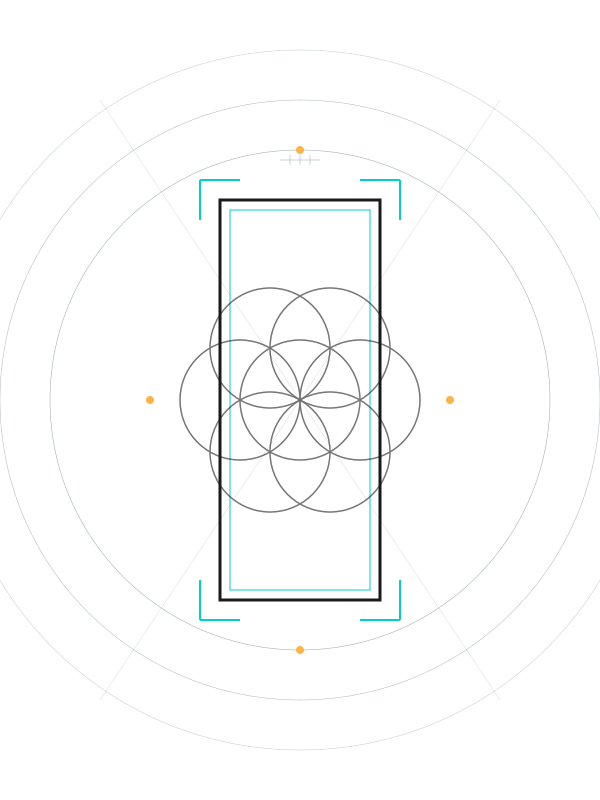
\includegraphics[width=4in]{artwork-intro.svg}
\end{center}

\vspace{0.4in}

\noindent This book is not theory. It's documentation.

Block A introduced you to the frameworks of self-actualization—the maps and models that help us understand consciousness evolution. Block B showed you how those frameworks manifest in practice through real stories of transformation.

Block C is different. This is the laboratory.

The raw material. The moments when consciousness breaks through barriers in real-time. The experiments we're running on ourselves while documenting the process for anyone brave enough to follow.

What you're about to read comes from two people actively experimenting with consciousness evolution—using technology, awareness, and pattern recognition to transform while the transformation is happening. We're not gurus who figured it all out and are now teaching from the mountaintop. We're researchers mid-experiment, sharing observations as we discover them.

This is messier than theory. More honest than inspiration. And more useful than either.

% ... [Content continues - would insert the full converted content here]

\end{document}
